\documentclass[10pt,a4paper]{article}

\usepackage[utf8]{inputenc}
\usepackage[margin=1in]{geometry}
\thispagestyle{empty}

\usepackage{amsmath}
\usepackage{amsfonts}
\usepackage{amssymb}

\usepackage{parskip}

\usepackage{listings}
\usepackage{xcolor}

\usepackage{enumerate}

\usepackage{hyperref}

\usepackage{float}
\restylefloat{figure}
\usepackage[font=small,labelfont=bf]{caption}
\usepackage{wrapfig}
Gaga
\usepackage{graphicx}
\restylefloat{figure}

\usepackage{cancel}

\usepackage{multicol}
\setlength{\columnsep}{22pt}

\usepackage{colortbl}

\usepackage{cases}

\usepackage{verbatim}

\title{Redes y Comunicaciones de Datos II}
\author{Cristian Escudero \\ \small{Resumen 2}}

\begin{document}
\maketitle

\section{La Capa de Red}

\subsection{NAT y PAT}

\subsubsection{NAT - Traducción de Dirección de Red (\textit{Network Adress Translation})}

Las direcciones IP son escasas. Si tiene más clientes que IPs, tiene un problema. Para clientes propios con las conexiones de línea conmutada, una manera de resolver el problema es asignar dinámicamente una dirección IP a una computadora cuando ésta llama e inicia la sesión, y tomar de vuelta la dirección IP cuando se termina la sesión y reasignarla a otra visita.

Esta estrategia falla para ISPs que sirven a una gran cantidad de usuarios, y más aún, si estos están conectados permanentemente a la red. La solución temporal que se designó hasta la transición a IPv6 fue la \textbf{Traducción de Dirección de Red} (\textbf{NAT}).

La idea básica de NAT es asignar un rango de direcciones IP públicas pequeño a cada compañía para el tráfico de Internet. \textbf{Dentro} de la compañía, cada computadora tiene una dirección IP única que se usa para enrutar el tráfico interno. Sin embargo, cuando un paquete sale de la compañía y va al ISP, se presenta una \textbf{traducción de dirección}. Para hacer posible este esquema existen tres rangos de direcciones IP que se han declarado como privados, que las compañías pueden usar internamente cuando lo deseen. La única regla es que ningún paquete que contiene estas direcciones puede aparecer en la propia Internet. De esta manera simultáneamente sólo pueden salir a Internet con una dirección IP pública tantos equipos como direcciones públicas se hayan contratado.

\begin{wrapfigure}{r}{0.5\textwidth}
  \caption{Los tres rangos de IPs reservadas.}
  \label{fig:ips_reservada}
  \centering
  \hbox{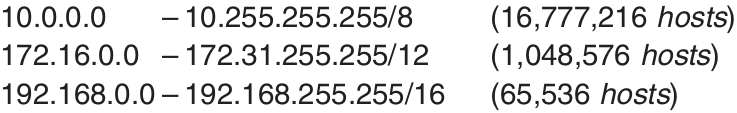
\includegraphics[width=0.45\textwidth-\fboxrule-\fboxrule]{imgs/ips_reservada.png}}
\end{wrapfigure}

Dentro de las instalaciones de la compañía, cada máquina tiene una dirección única privada. Sin embargo, cuando un paquete sale de las instalaciones de la compañía, pasa a través de una caja NAT que convierte la dirección interna de origen de IP, a una dirección IP pública de la compañía. A menudo, la caja NAT se combina en un solo dispositivo con un \textbf{firewall} (servidor de seguridad) que proporciona seguridad controlando cuidadosamente lo que entra y sale de la compañía.

\begin{figure}[!ht]
  \caption{Colocación y funcionamiento de una caja NAT.}
  \label{fig:nat}
  \centerline{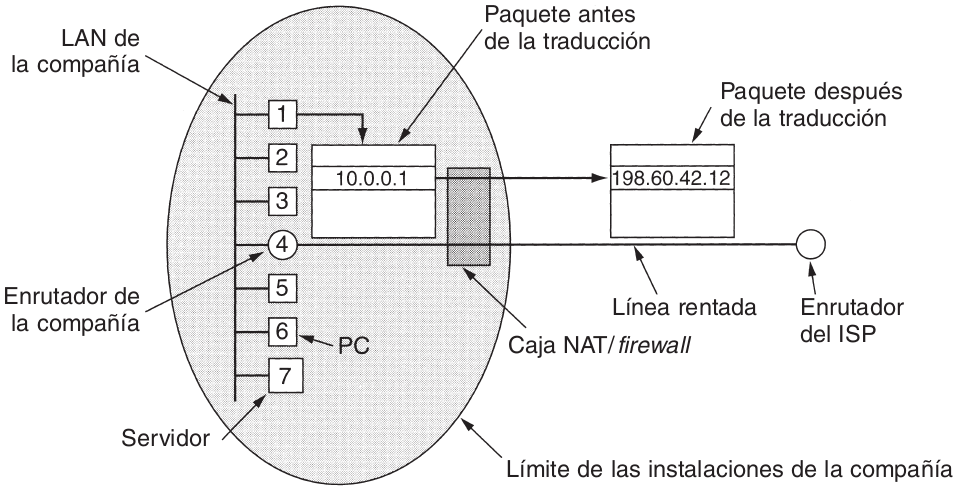
\includegraphics[width=0.8\textwidth-\fboxrule-\fboxrule]{imgs/nat.png}}
\end{figure}

En NAT, el enrutador sigue la pista de los datos básicos de cada conexión activa. Cuando una respuesta llega al enrutador, utiliza los datos de seguimiento de la conexión almacenados en la fase de salida para determinar la dirección privada de la red interna a la que remitir la respuesta.

\textit{¿Qué se hace cuándo se posee un rango muy pequeño o único de IPs públicas?} El problema realmente surge cuando dos o más \textit{hosts} se conectan a una misma IP. Para evitar la ambiguedad en el retorno, se introdució la \textbf{Traducción de Direcciones por Puerto} (\textbf{PAT}).

Siempre que un paquete \textbf{saliente} entra en la caja NAT (con PAT), además de modificarse la \textit{dirección de origen}, se modifica el campo \textit{Puerto de origen} TCP por un índice en la \textbf{tabla de traducción} de la caja NAT que almacena ambos valores.

Cuando un paquete \textbf{llega} a la caja NAT desde el ISP, el \textit{Puerto de origen} en el encabezado TCP del paquete se extrae y se obtiene la dirección de origen dentro de la red utilizando el respectivo índice de la tabla de traducción de la caja NAT.

¿\textit{Por qué usa un número de índice en una tabla en vez de directamente el valor del puerto origen}? Para evitar ambigüedades entre múltiples \textit{hosts} que usan el mismo valor de puerto.

El esquema de PAT puede ser utilizado directamente por los ISP para aliviar el problema de la escasez de IPs, consideranto a todos sus usuarios como una compañía grande, y brindándoles direcciones privadas.

\pagebreak
\section{La Capa de Aplicación}

Las capas por debajo de la de \textbf{aplicación} están ahí para proporcionar \textbf{transporte confiable}, pero no hacen ningún trabajo verdadero para los usuarios. En la CdA se necesitan protocolos de apoyo que permitan el funcionamiento de las aplicaciones reales. Uno de ellos es el \textbf{DNS} (\textit{Domain Name System}), que maneja la asignación de nombres dentro de Internet, facilitando el manejo de las direcciones de IP.

\subsection{DNS - El Sistema de Nombres de Dominio}

Dada a la dificultad de memorizar direcciones de red, y de la inflexibilidad de manejar cambios en las direcciones de los servidores al enviar mensajes a IPs, se introdujeron los nombres ASCII, con el fin de separar los \textbf{nombres de máquina} de las \textbf{direcciones de máquina}. Sin embargo, la red sólo comprende direcciones numéricas, por lo que se requieren algunos mecanismos para convertir las cadenas ASCII de nuevo a direcciones de red.

Una alternativa que surgió fue la de mantener un servidor con un archivo \textit{hosts.txt} que listaba todos los \textit{hosts} y sus direcciones de IP, y que se enviaba periódicamente a todos los \textit{hosts} de la red. 

Sin embargo, este método no sería práctico ante la presencia de miles de \textit{hosts}, ya que no solo el tamaño del archivo crecería de manera considerable, sino que además ocurrirían conflictos constantes con los nombres de los \textit{hosts} a menos de que dichos nombres se administraran \textbf{centralmente}, algo impensable en una red internacional enorme. Para resolver estos problemas, se inventó el \textbf{DNS}.

El DNS se basa en un esquema jerárquico que permite asignar nombres, basándose en el concepto de \textbf{dominio}, utilizando para su gestión una \textit{base de datos} (\textit{BD}) distribuida.

Para relacionar un nombre con una dirección IP, un programa de aplicación llama a un procedimiento de biblioteca llamado \textbf{resolvedor}, y le pasa el nombre como parámetro (\textbf{consulta DNS}). El resolvedor envía un paquete UDP a un servidor DNS local, que después busca el nombre y devuelve la dirección IP al resolvedor, que entonces lo remite al solicitante. Una vez que tiene la dirección IP, el programa puede establecer una conexión TCP con el destino, o enviarle paquetes UDP.

\subsubsection{El espacio de nombres del DNS}

Conceptualmente, Internet se divide en 200 \textbf{dominios} de nivel superior, cada uno de los cuales abarca muchos \textit{hosts}. Cada dominio se divide en \textbf{subdominios}, los cuales, a su vez, también se dividen, y así sucesivamente. Puede verse como un árbol, cuyas hojas representan los dominios que no tienen subdominios, y que además pueden contener un solo \textit{host}, o miles (si representa una organización).

Los dominios de nivel superior se dividen en dos categorías: \textbf{genéricos} y \textbf{de país} (o \textit{geográficos}).

\begin{figure}[ht!]
  \caption{Parte del espacio de nombres de dominio de Internet.}
  \label{fig:DNS_espacio_nombres}
  \centerline{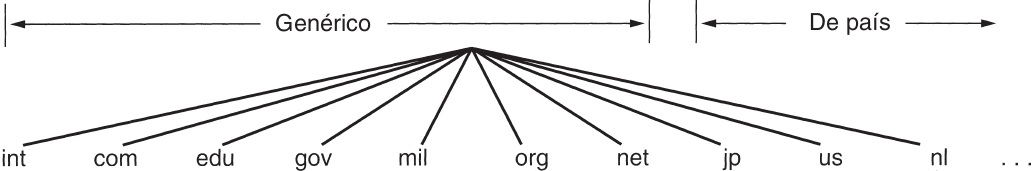
\includegraphics[width=0.9\textwidth-\fboxrule-\fboxrule]{imgs/DNS_espacio_nombres.png}}
\end{figure}

Cada dominio se nombra por la ruta hacia arriba desde él a la \textbf{raíz} (\textit{sin nombre}). Los componentes se separan con puntos (ej, ``\textit{eng.sun.com.}'').

Los \textbf{nombres de dominio} pueden ser:
\begin{itemize}
\item \textbf{Absolutos:} terminan con punto (ej, ``\textit{eng.sun.com.}'').
\item \textbf{Relativos:} tienen que interpretarse en algún contexto para determinar de manera única su significado verdadero (ej, ``\textit{eng.sun.com}'').
\end{itemize}

En ambos casos, un nombre de dominio hace referencia a un nodo específico del árbol y a todos los nodos por debajo de él, y no hacen distinción entre mayúsculas y minúsculas. Los nombres reflejan los \textbf{límites organizacionales}, no las redes físicas.

Para crear un nuevo dominio, se requiere el permiso del dominio en el que se incluirá, evitando así los conflictos de nombres y permitiendo a cada dominio llevar el registro de todos sus subdominios. Una vez que se ha creado y registrado un nuevo dominio, este puede crear subdominios, sin obtener el permiso de nadie más arriba en el árbol.

\subsubsection{Registros de recursos}

Cada dominio, sea un \textit{host} individual o un dominio de nivel superior, puede tener un grupo de \textbf{registros de recursos} (RRs) asociados a él. En un \textit{host} individual, el RR más común es simplemente su dirección IP, pero también existen muchos otros tipos de RRs. Cuando un resolvedor da un nombre de dominio al DNS, lo que recibe son los RRs asociados a ese nombre. Por lo tanto, DNS relaciona los dominios de nombres con los RRs.

Cada entrada en la tabla de un DNS contiene información, no sólo de las direcciones IP, si no de un RR, de cinco campos:

\begin{itemize}
\item \texttt{Nombre\_dominio:} el dominio al que pertenece ese registro. Puede haber más de un registro por dominio. Si se omite, se usa por defecto el último nombre de domino
indicado.
\item \texttt{TTL:} indica la estabilidad del registro.
\subitem + La información \textbf{altamente estable} tiene un valor grande (86.400 [seg], o sea, 1 día).
\subitem + La información \textbf{volátil} recibe un valor pequeño (60 [seg]).
\item \texttt{Clase:} para la información de Internet, siempre es \texttt{IN}. Si se omite, se toma el último valor indicado.
\item \texttt{Tipo:} indica el tipo de registro de que se trata.
\item \texttt{Valor:} puede ser un número, un nombre de dominio o una cadena ASCII. La semántica depende del tipo de registro.
\end{itemize}

\underline{\textbf{Principales tipos de RR DNS:}}

\begin{tabular}{rl p{10.5cm}}
{\bf Tipo} & {\bf Significado} & {\bf Descripción} \\\hline \\ [-1.5ex]
\texttt{SOA} &
\textit{Start of Autority} &
Inicio de autoridad, identificando el dominio o la zona. Fija una serie de parámetros para esta zona.
\\ [1ex] \hline \\ [-1.5ex]
%%%%%%%%%%%%%%%%%%%%%%%%%%
\textbf{\texttt{A}} &
\textit{Address} &
Dirección IP de un \textit{host} en 32 \texttt{bits}. Si este tiene varias direcciones IP, habrá un registro diferente por cada una de ellas.
\\ [1ex] \hline \\ [-1.5ex]
%%%%%%%%%%%%%%%%%%%%%%%%%%
\texttt{MX} &
\textit{Mail eXchanger} &
Especifica el nombre del dominio que está preparado para aceptar correo electrónico.
\\ [1ex] \hline \\ [-1.5ex]
%%%%%%%%%%%%%%%%%%%%%%%%%%
\texttt{NS} &
\textit{Name Server} &
El nombre de dominio se hace corresponder con el nombre de una computadora de confianza para el dominio o servidor de nombres.
\\ [1ex] \hline \\ [-1.5ex]
%%%%%%%%%%%%%%%%%%%%%%%%%%
\texttt{CNAME} &
\textit{Canonical Name} &
Es un alias que se corresponde con el nombre canónico verdadero.
\\ [1ex] \hline \\ [-1.5ex]
%%%%%%%%%%%%%%%%%%%%%%%%%%
\texttt{PTR} &
\textit{Pointer} &
Apuntador, hace corresponder una dirección IP con el nombre de un sistema. Usado para asociar \{\texttt{dirección IP, nombre}\}, y realizar de esa forma \textbf{búsquedas inversas}.
\\ [1ex] \hline \\ [-1.5ex]
%%%%%%%%%%%%%%%%%%%%%%%%%%
\texttt{HINFO} &
\textit{Host Info} &
Información del \textit{host}, tipo y modelo de computadora y SO, en ASCII.
\\ [1ex] \hline \\ [-1.5ex]
%%%%%%%%%%%%%%%%%%%%%%%%%%
\texttt{TXT} &
\textit{Text} &
Texto ACII no interpretado. Permite agregar comentarios a la BD.
\\ [1ex] \hline \\ [-1.5ex]
%%%%%%%%%%%%%%%%%%%%%%%%%%
\texttt{WKS} &
\textit{Well-Known Services} &
Servicios públicos. Puede listar los servicios de las aplicaciones disponibles en el ordenador.
\\ [1ex] \hline \\ [-1.5ex]
%%%%%%%%%%%%%%%%%%%%%%%%%%
\end{tabular}

\subsubsection{Servidores de nombres}

Un \textbf{solo} servidor de nombres podría contener toda la BD DNS y responder a todas las consultas dirigidas a ella, pero estaría tan sobrecargado que sería inservible. Más aún, si llegara a caerse, la Internet completa se vendría abajo.

Para evitar los problemas asociados a tener una sola fuente de información, el espacio de nombres DNS se divide en \textbf{zonas} no traslapantes. Una zona es una parte contigua del \textbf{árbol de nombres} que se administra como una unidad.

Cuando un resolvedor tiene una consulta referente a un nombre de dominio, la pasa a uno de los servidores de nombres locales. Si el dominio que se busca cae bajo la jurisdicción del servidor de nombres, devuelve los registros de \textbf{recursos autorizados} -que provienen de la autoridad que administra el registro y, por lo tanto, siempre son correctos-. Los registros autorizados contrastan con los \textbf{registros en caché}, que podrían no estar actualizados.

Por otro lado, si el dominio es remoto y no hay información disponible localmente sobre el dominio solicitado, el servidor de nombres envía un mensaje de consulta al servidor de nombres de nivel superior en el que le solicita dicho dominio.

Este método de consultas conoce como \textbf{consulta recursiva}, puesto que cada servidor que no tiene toda la información solicitada la busca en algún otro lado y luego la proporciona. Algunos servidores no implementan este método y siempre devuelven el nombre del siguiente servidor a intentar (\textbf{consulta iterativa}).

Cuando un cliente DNS no recibe una respuesta antes de que termine su temporizador, por lo general probará con otro servidor la siguiente vez, asumiendo que el servidor probablemente esté inactivo.

Otro método es el de \textbf{búsqueda inversa}, que dado una dirección IP, devuelve el nombre. Para evitar una búsqueda exhaustiva por todo el espacio de nombres de dominio, se utiliza un dominio especial llamado \texttt{in-addr.arpa}. Cuando un cliente DNS desea conocer el nombre de dominio asociado a la dirección IP $w.x.y.z$ realiza una pregunta inversa a \texttt{z.y.x.w.in-addr.arpa}.

\underline{Nota:} la inversión de los \texttt{bytes} es necesaria debido a que los nombres de dominio son más genéricos por la derecha, al contrario que ocurre con las direcciones IP.

\underline{\textbf{Tipos de servidores:}}

\begin{enumerate}
\item \textbf{Primarios (\textit{Primary Name Servers}):} almacenan la información de su zona en una BD local. Son responsables de mantener la información actualizada y cualquier cambio debe ser notificado a este servidor.
\item \textbf{Secundarios (\textit{Secundary Name Servers}):} obtienen los datos de su zona desde otro servidor que tenga autoridad para esa zona. El proceso de copia de la información se denomina \textbf{transferencia de zona}.
\item \textbf{Maestros (\textit{Master Name Servers}):} transfieren las zonas a los servidores secundarios. Cuando un servidor secundario arranca busca un servidor maestro y realiza la \textit{transferencia de zona}. Un servidor maestro para una zona puede ser a la vez un servidor primario o secundario de esa zona. Estos servidores extraen la información desde el servidor primario de la zona. Así se evita que los servidores secundarios sobrecargen al servidor primario con transferencias de zonas.
\item \textbf{Locales (\textit{Caching-only servers})}: no tienen autoridad sobre ningún dominio; se limitan a contactar con otros servidores para resolver las peticiones de los clientes DNS. Estos servidores mantienen una memoria caché con las últimas preguntas contestadas. Cada vez que un cliente DNS le formula una pregunta, primero consulta en su memoria caché. Si encuentra la dirección IP solicitada, se la devuelve al cliente; si no, consulta a otros servidores, apuntando la respuesta en su memoria caché y comunicando la respuesta al cliente.
\item \textbf{Raíz (``.''):} se usa para consultar \textit{hosts} externos, cuyas direcciones IP están presentes en un fichero de configuración del sistema y se cargan en el caché del DNS al iniciar el servidor. Proporcionan referencias directas a
servidores de los dominios de segundo nivel (COM, EDU, geográficos, étc). Conocen a todos los servidores de dominios de primer nivel. Reciben consultas de servidores locales que no saben resolver un nombre. Hay trece servidores raíz a lo largo del mundo.
\end{enumerate}

\subsection{Correo Electrónico}

Los primeros sistemas de correo electrónico simplemente consistían en protocolos de transferencia de archivos, conteniendo la primera línea del archivo la dirección del destinatario.

Algunas limitaciones que surgieron de este sistema:
\begin{itemize}
\item envío a grupos;
\item sin notificación de entrega;
\item sin estructura interna de envío.
\end{itemize}

En 1982 se publicaron las propuestas de correo electrónico del ARPANET:
\begin{itemize}
\item \texttt{RFC 821.} Protocolo de transmisión SMTP.
\item \texttt{RFC 822.} Formato de mensaje.
\end{itemize}

El CCITT elaboró su recomendación \texttt{X.400} para reemplazar al \texttt{RFC 822}, pero su excesiva complejidad lo hizo desaparecer, como le sucedió a la mayoría de las aplicaciones OSI.

\subsubsection{Arquitectura y servicios}

Los sistemas de correo electrónico normalmente consisten en dos subsistemas:

\begin{itemize}
\item Los \textbf{agentes de usuario}, que permiten leer y enviar correo electrónico. Son programas locales para interactuar con el sistema de correo electrónico. El usuario debe proporcionar el mensaje, la dirección de destino (en un formato que el agente de usuario pueda manejar, como direcciones DNS de la forma \textit{example@dns-address}) y, posiblemente, algunos otros parámetros.
\item Los \textbf{agentes de transferencia de mensajes}, que mueven los mensajes del origen al destino. Son por lo común \textit{daemons} del sistema que operan en segundo plano y mueven correo electrónico a través del sistema. Se clasifican a su vez en:
\subitem + \textbf{De distribución.} (SMTP, ESMTP).
\subitem + \textbf{De entrega final.} (POP3, IMAP).
\end{itemize}

Por lo general,los sistemas de correo electrónico desempeñan cinco funciones básicas:

\begin{enumerate}
\item La \textbf{redacción} se refiere al proceso de crear mensajes y respuestas. 
\item La \textbf{transferencia} se refiere a mover mensajes del remitente al destinatario. Requiere establecer una conexión con el destino o alguna máquina intermedia, enviar el mensaje y liberar la conexión, todo de forma automática.
\item La \textbf{generación del informe} notifica que ocurrió con el mensaje: \textit{¿se entregó, rechazó o se perdió?}
\item La \textbf{visualización} de los mensajes es necesaria para que la gente pueda leer su correo electrónico. 
\item La \textbf{disposición} tiene que ver con lo que el destinatario hace con el mensaje una vez que lo recibe.
\end{enumerate}

En los sistemas de correo electrónico, existe una clara distinción entre el \textbf{sobre} (\texttt{RFC 821}) y su \textbf{contenido} (\texttt{RFC 822}). El sobre encapsula el mensaje; contiene toda la información necesaria para transportar el mensaje, como dirección de destino, prioridad y nivel de seguridad, la cual es diferente del mensaje mismo. Los agentes de transporte del mensaje usan el sobre para enrutar.

El mensaje dentro del sobre contiene dos partes: el \textbf{encabezado}, que contiene información de control para los agentes de usuario, y el \textbf{cuerpo}, que es por completo para el destinatario humano.

\subsubsection{Formatos de mensaje}

\underline{\textbf{RFC 822:}}

Los mensajes consisten en un sobre primitivo, algunos campos de encabezado, una línea en blanco y el cuerpo del mensaje. Cada campo de cabecera consiste en una sola línea de
texto ASCII que contiene el nombre del campo, dos puntos (:), y, para la mayoría de los campos, un valor.

\begin{figure}[ht!]
  \caption{Campos de encabezado \texttt{RFC 822}: relacionados con el transporte de mensajes (\textit{arriba}); usados por los agentes de usuario o destinatarios (\textit{abajo}).}
  \label{fig.:encabezado_RFC822}
  \centerline
  {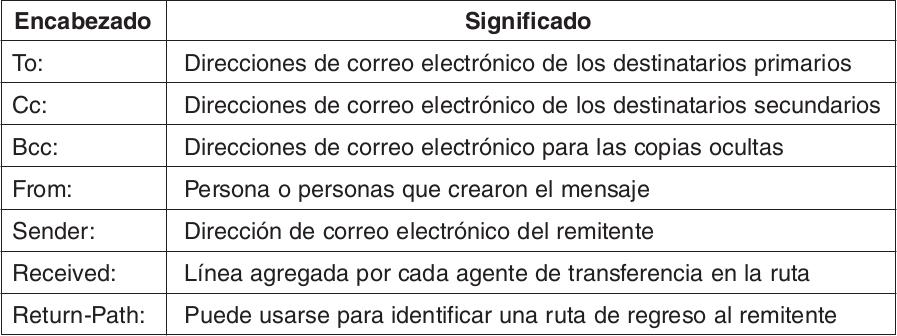
\includegraphics[width=.65\textwidth-\fboxrule-\fboxrule]{imgs/encabezado_RFC822.png}}
  \vspace{10pt}
  \centerline
  {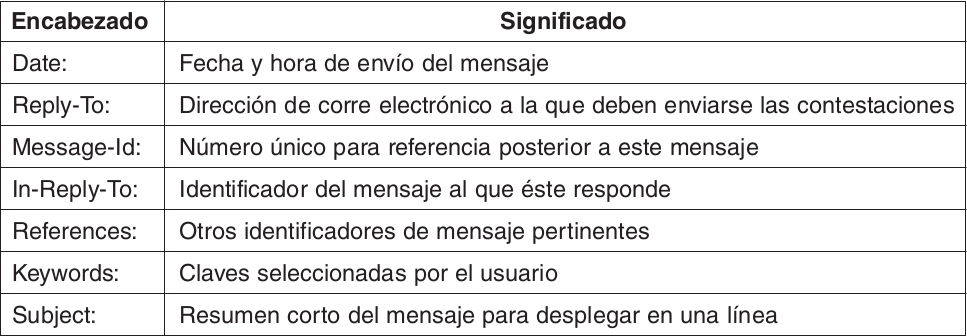
\includegraphics[width=.65\textwidth-\fboxrule-\fboxrule]{imgs/encabezado_RFC822_2.png}}  
\end{figure}

El \texttt{RFC 822} explícitamente indica que los usuarios pueden inventar cabeceras nuevas para uso privado siempre y cuando comiencen con la cadena \texttt{X-}.

\underline{\textbf{MIME - Extensiones Multipropósito de Correo de Internet}}

La idea básica de MIME es continuar usando el formato \texttt{RFC 822}, pero agregar una estructura al cuerpo del mensaje y definir reglas de codificación para los mensajes no ASCII. De esa manera, nada cambia de la arquitectura anterior del \texttt{RFC 822}. Sólo afecta a los agentes de usuario, ya que para SMTP es totalmente transparente.

MIME define cinco nuevos encabezados de mensaje:

\begin{tabular}{r p{10.5cm}}
{\bf Encabezado} & {\bf Significado} \\\hline \\ [-1.5ex]
\texttt{MIME-Version} &
Identifica la version de MIME. Si no existe se considera que el mensaje es texto normal en inglés.
\\ [1ex] \hline \\ [-1.5ex]
%%%%%%%%%%%%%%%%%%%%%%%%%%
\texttt{Content-Description} &
Cadena de texto que describe el contenido. Esta cadena es necesaria para que el destinatario sepa si desea descodificar y leer el mensaje o no.
\\ [1ex] \hline \\ [-1.5ex]
%%%%%%%%%%%%%%%%%%%%%%%%%%
\texttt{Content-Id} &
Identificador único, usa el mismo formato que el encabezado estándar \texttt{Message-Id}.
\\ [1ex] \hline \\ [-1.5ex]
%%%%%%%%%%%%%%%%%%%%%%%%%%
\texttt{Content-Transfer-Encoding} &
Indica la manera en que está envuelto el cuerpo del mensaje. Existen cinco tipos básicos de \textbf{esquemas} de codificación de mensajes: \texttt{ASCII 7}, \texttt{ASCII 8}, \textit{codificación binaria}, \texttt{base64}, y \textit{codificación entrecomillada imprimible}.
\\ [1ex] \hline \\ [-1.5ex]
%%%%%%%%%%%%%%%%%%%%%%%%%%
\texttt{Content-Type} &
Especifica la naturaleza del cuerpo del mensaje. Existen 7 tipos básicos (\textit{text, image, audio, video, application, message, multipart}), cada uno de los cuales tiene uno o más subtipos. El \textit{tipo} y el \textit{subtipo} se separan mediante un carácter diagonal (/). Ejemplo: \texttt{video/mpeg}.
\\ [1ex] \hline \\ [-1.5ex]
%%%%%%%%%%%%%%%%%%%%%%%%%%
\end{tabular}

\subsubsection{Transferencia de mensajes}

\underline{\textbf{SMTP - Protocolo Simple de Transporte de Correo}}

SMTP es un protocolo ASCII sencillo \textbf{cliente/servidor}. El correo electrónico se entrega al hacer que la máquina de origen establezca una conexión TCP con el \textbf{puerto 25} de la máquina de destino. Escuchando en este puerto está un \textit{daemon} de correo electrónico que habla con el SMTP. Este \textit{daemon} acepta conexiones de entrada y copia mensajes de estas a los buzones adecuados. Si no puede entregarse un mensaje, se devuelve al remitente un informe de error que contiene la primera parte del mensaje que no pudo entregarse.

Después de establecer la conexión TCP con el puerto 25, el servidor comienza por enviar una línea de texto que proporciona su identidad e indica si está preparado o no para recibir correo:

\begin{itemize}
\item Si \textbf{no está dispuesto}, el cliente libera la conexión y lo intenta después.
\item Si \textbf{está dispuesto}, el cliente anuncia de quién proviene el mensaje, y a quién está dirigido. Si existe el destinatario en el destino, el servidor da al cliente permiso para enviar el mensaje. A continuación el cliente envía el mensaje y el servidor confirma su recepción. Una vez que todo el correo electrónico ha sido intercambiado en \textbf{ambas direcciones}, se libera la conexión.
\end{itemize}

Aunque el protocolo SMTP está bien definido, pueden surgir algunos problemas:

\begin{itemize}
\item La longitud del mensaje en implementaciones viejas de SMTP está limitada a \texttt{64 Kb}.
\item Si el cliente y el servidor tienen temporizaciones distintas, uno de ellos puede terminar mientras que el otro continúa trabajando, terminando inesperadamente la conexión.
\end{itemize}

Para superar algunos de estos problemas, se ha definido el \textbf{SMTP extendido} (\textbf{ESMTP}).

\subsubsection{Entrega final}

\begin{description}
\item \textbf{Problema:} acceso no permanente a internet, por ende, no se puede enviar correo directo entre \textit{hosts}.
\item \textbf{Solución:} que un agente de transferencia de mensajes en una máquina ISP acepte correo electrónico para sus clientes y lo almacene en sus buzones en una máquina ISP con acceso permanente.
\end{description}

Un cliente puede consultar su buzón en la máquina ISP a través de los siguientes protocolos:

\begin{itemize}
\item \textbf{POP3 (Post Office Protocol):} tiene comandos para que un usuario establezca una sesión (\texttt{USER} y \texttt{PASS}), la termine (\texttt{QUIT}), obtenga mensajes (\texttt{RETR}) y los borre (\texttt{DELE}). El protocolo mismo consiste en texto ASCII y se asemeja a SMTP. Su objetivo es obtener el correo electrónico del buzón remoto y almacenarlo en la máquina local del usuario para su lectura posterior. Usa el \textbf{puerto 110}.
\item \textbf{IMAP (Interactive Mail Access Protocol):} la idea en que se basa es que el servidor de correo electrónico mantenga un depósito central al que puede accederse desde
cualquier máquina. Por tanto, a diferencia del POP3, no descarga el correo electrónico en la máquina personal del usuario dado que el usuario puede tener varias computadoras para consultar el correo. Además verifica si los correos ya han sido leídos con anterioridad. Usa el \textbf{puerto 143}.
\end{itemize}

\subsection{World Wide Web}

Acceso a documentos multimedia vinculados (\textbf{hipervínculos}) distribuidos en Internet. Posee un modelo \textbf{cliente/servidor}. 

\begin{multicols}{2}
\raggedcolumns

En el cliente:
\begin{itemize}
\item navegador (\textit{browser}) para mostrar información recibida 
\item establece una conexión \textit{telnet} al \textbf{puerto 80} del servidor y envía comandos para recuperar información.
\end{itemize}

\columnbreak

En el servidor:
\begin{itemize}
\item proceso TCP de escucha en \textbf{puerto 80}.
\item Una vez recibida una solicitud de un cliente, se envía respuesta y se libera la conexión.
\end{itemize}

\end{multicols}

Las \textbf{solicitudes} son en formato ASCII, y las \textbf{respuestas} son mensajes estructurados tipo MIME. Esto es según el protocolo \textbf{HTTP} (\textit{HyperText Transfer Protocol}).

\underline{\textbf{Cookies:}}

Una cookie es un pequeño archivo (o cadena, de a lo mucho \texttt{4 KB}). Los navegadores almacenan \textit{cookies} ofrecidas en un \textit{directorio de cookies} en el disco duro de la máquina del cliente (a menos que el usuario las haya deshabilitado).

Una cookie puede contener hasta cinco campos:

\begin{itemize}
\item \texttt{Dominio:} indica de dónde viene la cookie. 
\item \texttt{Ruta:} es la ruta en la estructura del directorio del servidor que identifica qué partes del árbol de archivos del servidor podrían utilizar la cookie. Por lo general es (\texttt{/}), lo que significa el árbol completo.
\item \texttt{Contenido:} toma la forma \{\texttt{nombre = valor}\}, que pueden ser los
que el servidor desee.
\item \texttt{Expira:} especifica cuándo caduca la cookie. Si este campo está ausente, el navegador descarta la cookie cuando sale (\textbf{cookie no persistente}). Si se proporciona una hora y una fecha, se mantiene hasta que expira (\textbf{cookie persistente}).
\item \texttt{Seguro:} indica que el navegador podría simplemente regresar la cookie a un servidor seguro.
\end{itemize}

\subsubsection{Protocolos FTP y Telnet}

\underline{\textbf{FTP (\textit{File Transfer Protocol}):}}

Protocolo de transferencia de archivos, básico pero útil y fácil de usar. Disponible para muchos SO. Las funciones esenciales permiten:
\begin{itemize}
\item copiar archivos de un sistema a otro;
\item ver listados de directorios;
\item realizar tareas de gestión como cambiar de nombre o borrar archivos.
\end{itemize}

El \textbf{Trivial FTP} (\textbf{TFTP}) se utiliza en situaciones especiales como carga software (\textit{SOs}, por ejemplo) en equipos sin disco duro (por ejemplo, \textit{enrutadores}).

\underline{\textbf{Telnet (\textit{Terminal Networking})}}

Protocolo de acceso a un ordenador desde otro ordenador sobre TCP. Disponible para muchos SO incluidos. Su acceso es a través del \textbf{puerto 23}. Aunque se ideó para comunicaciones \textit{peer-to-peer} se usa para aplicaciones \textbf{cliente/servidor}. Por problemas de seguridad está siendo sustituido por el \textbf{SSH} (\textbf{Secure Shell}).

\subsubsection{Mejoras de desempeño}

\underline{\textbf{Almacenamiento en caché:}}

Una forma muy sencilla de mejorar el desempeño es guardar las páginas que han sido solicitadas en caso de que se utilicen nuevamente, es decir, \textbf{almacenarlas en caché}. Esta es una técnica en el \textbf{cliente}. El procedimiento común es que algún proceso, llamado \textbf{proxy}, mantenga el caché. Para utilizar el almacenamiento en caché, un navegador puede configurarse para que todas las solicitudes de páginas se le hagan a un proxy en lugar de al servidor real de la página. Si el proxy tiene la página, la regresa de inmediato. De lo contrario, la obtiene del servidor, la agrega al caché para uso posterior y la envía al cliente que la solicitó. Tiene que tener además una forma de determinar la obsolescencia de la página, y descartarla del caché luego de cierto tiempo (que dependerá de la estabilidad de la página).

\underline{\textbf{Replicación del servidor:}}

Es una técnica en el \textbf{servidor}. El método más común que los servidores utilizan para mejorar el desempeño es replicar su contenido en múltiples ubicaciones separadas considerablemente (\textbf{espejeo} ó \textit{mirroring}). De esa forma, se distribuye la carga en distintos servidores.


\end{document}
